\hypertarget{project-design-documentation}{%
\section{PROJECT Design
Documentation}\label{project-design-documentation}}

\begin{quote}
\emph{The following template provides the headings for your Design
Documentation. As you edit each section make sure you remove these
commentary `blockquotes'; the lines that start with a \textgreater{}
character and appear in the generated PDF in italics.}
\end{quote}

\hypertarget{team-information}{%
\subsection{Team Information}\label{team-information}}

\begin{itemize}
\tightlist
\item
  Team name: thePurpleNarwhals
\item
  Team members

  \begin{itemize}
  \tightlist
  \item
    Michael Taylor
  \item
    Greg Villafane
  \item
    Huan Huynh
  \item
    Andrew Chacon
  \end{itemize}
\end{itemize}

\hypertarget{executive-summary}{%
\subsection{Executive Summary}\label{executive-summary}}

The application must allow players to play checkers with other players
who are currently signed in. The game user interface (UI) will support a
game experience using drag-and-drop browser capabilities for making
moves. Beyond this minimal set of features, we have grand vision for how
we could further enhance the player experience with some additional
features beyond the basic checkers game.

\hypertarget{purpose}{%
\subsubsection{Purpose}\label{purpose}}

Create a web-based Checkers game using Maven and Freemarker,
implementing the game through frontend and backend development. Each
player should be able to successfully play a game of checkers.

\hypertarget{glossary-and-acronyms}{%
\subsubsection{Glossary and Acronyms}\label{glossary-and-acronyms}}

\begin{quote}
\emph{Provide a table of terms and acronyms.}
\end{quote}

\begin{longtable}[]{@{}ll@{}}
\toprule
Term & Definition \\
\midrule
\endhead
VO & Value Object \\
\bottomrule
\end{longtable}

\hypertarget{requirements}{%
\subsection{Requirements}\label{requirements}}

This section describes the features of the application.

\hypertarget{definition-of-mvp}{%
\subsubsection{Definition of MVP}\label{definition-of-mvp}}

\begin{itemize}
\tightlist
\item
  As a user I want to be able to sign in with the desired username of my
  choice.
\item
  As a user I want to be able to start a game and play with another.
\item
  As a user I want to be able to move a piece when I drag a piece to a
  valid square.
\item
  As a user I want to be able to capture a piece when I drag a piece
  over an opponent's piece.
\item
  As a user I want to be able to forfeit the game when I feel helpless
  to end the game.
\end{itemize}

\hypertarget{mvp-features}{%
\subsubsection{MVP Features}\label{mvp-features}}

\begin{quote}
\emph{Provide a list of top-level Epics and/or Stories of the MVP.}
\end{quote}

\hypertarget{roadmap-of-enhancements}{%
\subsubsection{Roadmap of Enhancements}\label{roadmap-of-enhancements}}

\begin{quote}
\emph{Provide a list of top-level features in the order you plan to
consider them.}
\end{quote}

\hypertarget{application-domain}{%
\subsection{Application Domain}\label{application-domain}}

This section describes the application domain.

\begin{figure}
\centering
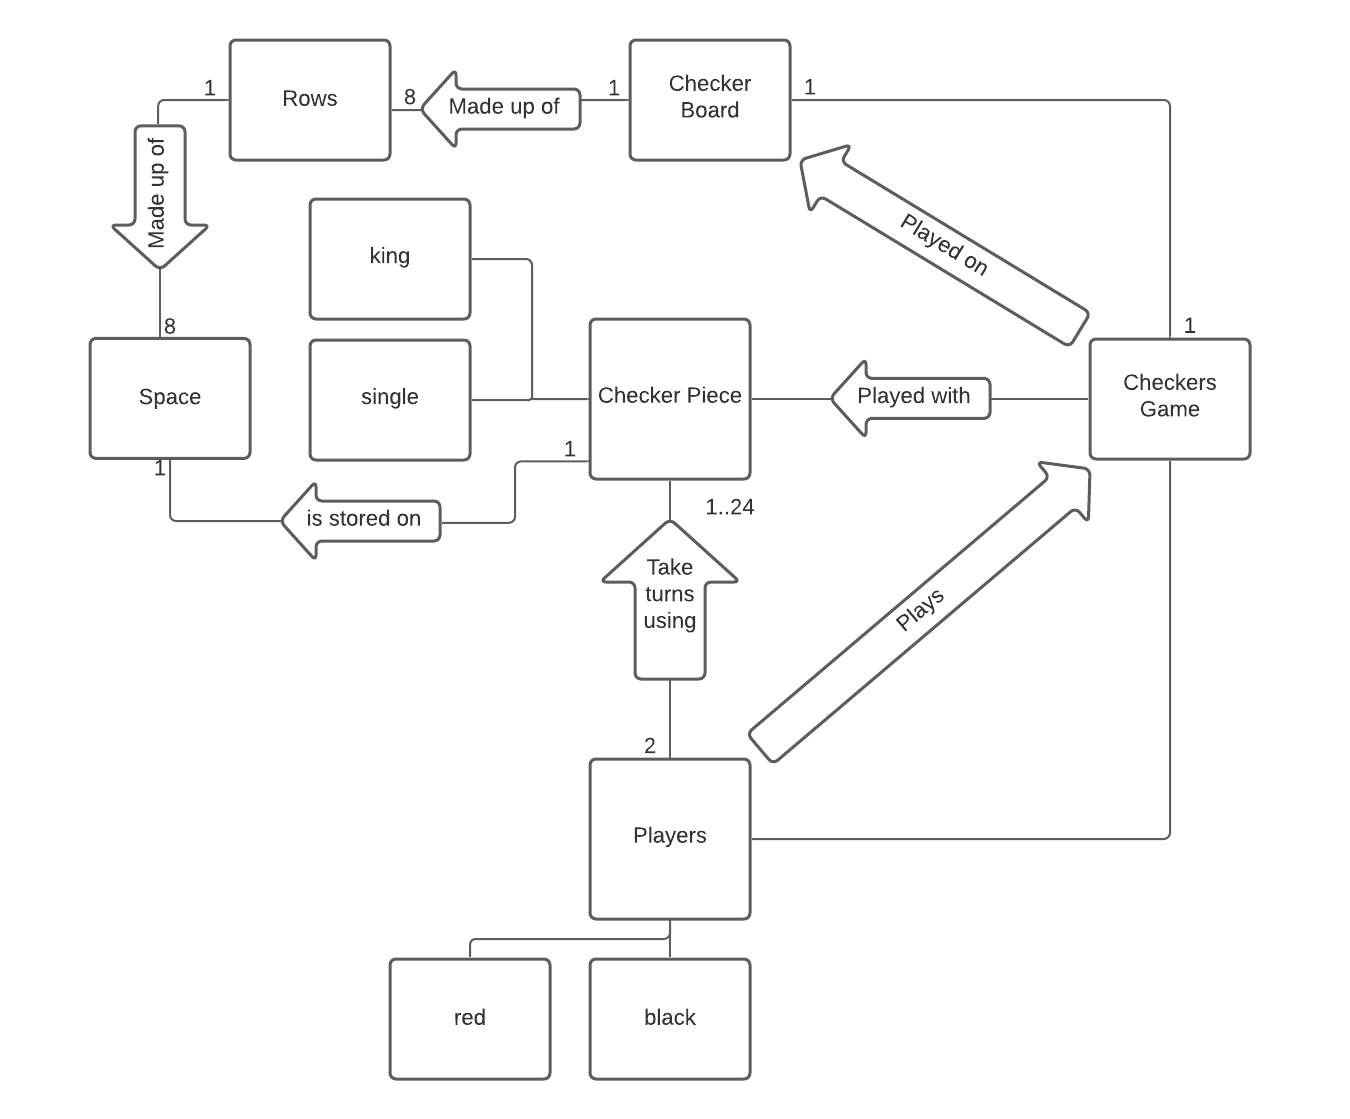
\includegraphics{domain-model.png}
\caption{The WebCheckers Domain Model}
\end{figure}

A Player will play a Checkers game, making the move using the pieces.
The Game has a Board for the game to be played on. The Board is made up
of Rows and Spaces, which the pieces will be stored on.

\hypertarget{architecture-and-design}{%
\subsection{Architecture and Design}\label{architecture-and-design}}

This section describes the application architecture.

\hypertarget{summary}{%
\subsubsection{Summary}\label{summary}}

The following Tiers/Layers model shows a high-level view of the webapp's
architecture.

\begin{figure}
\centering
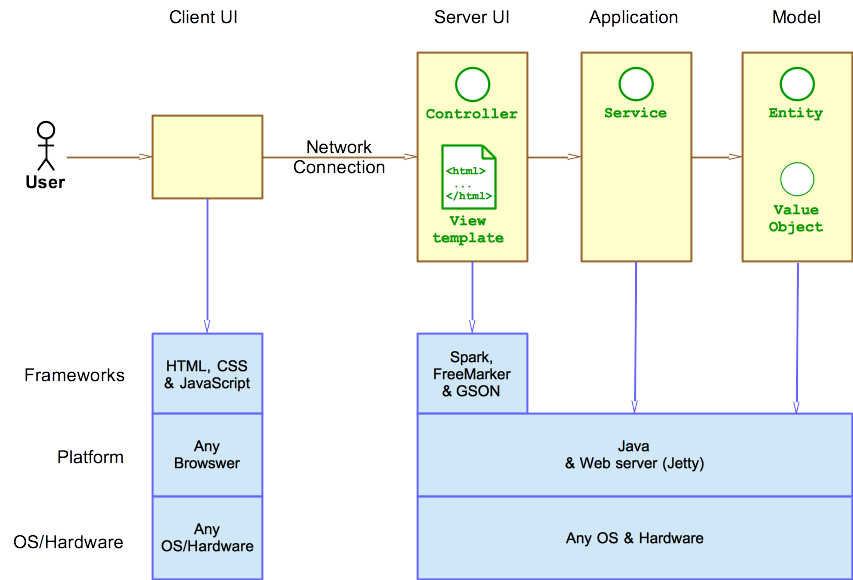
\includegraphics{architecture-tiers-and-layers.png}
\caption{The Tiers \& Layers of the Architecture}
\end{figure}

As a web application, the user interacts with the system using a
browser. The client-side of the UI is composed of HTML pages with some
minimal CSS for styling the page. There is also some JavaScript that has
been provided to the team by the architect.

The server-side tiers include the UI Tier that is composed of UI
Controllers and Views. Controllers are built using the Spark framework
and View are built using the FreeMarker framework. The Application and
Model tiers are built using plain-old Java objects (POJOs).

Details of the components within these tiers are supplied below.

\hypertarget{overview-of-user-interface}{%
\subsubsection{Overview of User
Interface}\label{overview-of-user-interface}}

This section describes the web interface flow; this is how the user
views and interacts with the WebCheckers application.

\begin{figure}
\centering
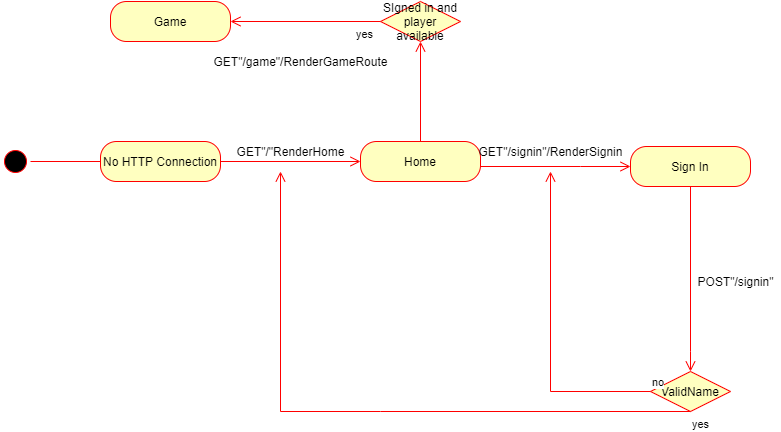
\includegraphics{web-interface.png}
\caption{The WebCheckers Web Interface Statechart}
\end{figure}

The user will go to the home page when first coming to the application.
The user will then be able to get to the /signin page. If the name
entered is valid, then they will be taken to the /home page. If the name
entered is invalid, then they will stay at the /signin page. When the
user is signed in and at the home page, the user will then be able to
get to the /game page to play a game.

\hypertarget{ui-tier}{%
\subsubsection{UI Tier}\label{ui-tier}}

\begin{quote}
\emph{Provide a summary of the Server-side UI tier of your architecture.
Describe the types of components in the tier and describe their
responsibilities. This should be a narrative description, i.e.~it has a
flow or ``story line'' that the reader can follow.}
\end{quote}

\begin{quote}
\emph{At appropriate places as part of this narrative provide one or
more static models (UML class structure or object diagrams) with some
details such as critical attributes and methods.}
\end{quote}

\begin{quote}
\emph{You must also provide any dynamic models, such as statechart and
sequence diagrams, as is relevant to a particular aspect of the design
that you are describing. For example, in WebCheckers you might create a
sequence diagram of the \texttt{POST\ /validateMove} HTTP request
processing or you might show a statechart diagram if the Game component
uses a state machine to manage the game.}
\end{quote}

\begin{quote}
\emph{If a dynamic model, such as a statechart describes a feature that
is not mostly in this tier and cuts across multiple tiers, you can
consider placing the narrative description of that feature in a separate
section for describing significant features. Place this after you
describe the design of the three tiers.}
\end{quote}

\hypertarget{application-tier}{%
\subsubsection{Application Tier}\label{application-tier}}

\begin{quote}
\emph{Provide a summary of the Application tier of your architecture.
This section will follow the same instructions that are given for the UI
Tier above.}
\end{quote}

\hypertarget{model-tier}{%
\subsubsection{Model Tier}\label{model-tier}}

\begin{quote}
\emph{Provide a summary of the Application tier of your architecture.
This section will follow the same instructions that are given for the UI
Tier above.}
\end{quote}

\hypertarget{design-improvements}{%
\subsubsection{Design Improvements}\label{design-improvements}}

\begin{quote}
\emph{Discuss design improvements that you would make if the project
were to continue. These improvement should be based on your direct
analysis of where there are problems in the code base which could be
addressed with design changes, and describe those suggested design
improvements. After completion of the Code metrics exercise, you will
also discuss the resutling metric measurements. Indicate the hot spots
the metrics identified in your code base, and your suggested design
improvements to address those hot spots.}
\end{quote}

\hypertarget{testing}{%
\subsection{Testing}\label{testing}}

\begin{quote}
\emph{This section will provide information about the testing performed
and the results of the testing.}
\end{quote}

\hypertarget{acceptance-testing}{%
\subsubsection{Acceptance Testing}\label{acceptance-testing}}

\begin{quote}
\emph{Report on the number of user stories that have passed all their
acceptance criteria tests, the number that have some acceptance criteria
tests failing, and the number of user stories that have not had any
testing yet. Highlight the issues found during acceptance testing and if
there are any concerns.}
\end{quote}

\hypertarget{unit-testing-and-code-coverage}{%
\subsubsection{Unit Testing and Code
Coverage}\label{unit-testing-and-code-coverage}}

\begin{quote}
\emph{Discuss your unit testing strategy. Report on the code coverage
achieved from unit testing of the code base. Discuss the team's coverage
targets, why you selected those values, and how well your code coverage
met your targets. If there are any anomalies, discuss those.}
\end{quote}
